\documentclass[a4paper]{exam}

\usepackage{geometry}
\usepackage{graphicx}
\usepackage{hyperref}
\usepackage{titling}

\printanswers

\title{Weekly Challenge 01: Comparison\\CS/MATH 113 Discrete Mathematics}
\author{$\langle team-name \rangle$}  % <== for grading, replace with your team name, e.g. q1-team-420
\date{Habib University | Spring 2023}

\qformat{{\large\bf \thequestion. \thequestiontitle}\hfill}
\boxedpoints

\begin{document}
\maketitle

\begin{questions}
  
\titledquestion{Safety at the Carnival}
  \begin{minipage}{.3\linewidth}
  \centerline{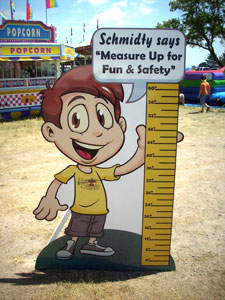
\includegraphics[width=\textwidth]{height}}
\end{minipage}
  \begin{minipage}{.65\linewidth}
Schmidty \cite{schmidt} has grown old and his vision is weak. He can no longer see if a person meets the height limit. The carnival organizers have installed a sensor to help. It beeps if any of the people in the waiting area is not eligible. Schmidty can move people in and out of the waiting area and then apply the sensor.

  \begin{parts}
  \part A family of 5 is trying to sneak in their toddler who does not meet the limit. Describe how Schmidty can identify the toddler in no more than 3 applications of the sensor.
  \part What is the smallest number of times that Schmidty needs to apply the sensor for a family of size $n$ in which only one person is below the limit. Justify your answer.
  \end{parts}
\end{minipage}
\begin{solution}
    % Enter your solution here.
  \end{solution}
\end{questions}

\begin{thebibliography}{9}
\bibitem{schmidt}
  TJ Schmidt \& Company (Standish, MI). \emph{Safety \& Maintenance}. \url{https://tjschmidtcarnival.com/pageserver/safety}. \textit{Last accessed on 6 Jan, 2023}.
\end{thebibliography}

\end{document}

%%% Local Variables:
%%% mode: latex
%%% TeX-master: t
%%% End: